\documentclass[12pt]{article}
\usepackage{scrextend}
\usepackage[utf8]{inputenc}
\usepackage[polish]{babel}
\usepackage[T1]{fontenc}%polskie znaki
\usepackage[utf8]{inputenc}%polskie znaki
\usepackage{geometry}
\usepackage{float}
\usepackage{enumitem}
\usepackage{hyperref}
\usepackage{graphicx}
\usepackage{amsmath}
\usepackage{tabularx}


\renewcommand{\baselinestretch}{1.5}


\begin{document}

\begin{flushleft}
    Damian Koper \textbf{241292} \\
\end{flushleft}
\vspace{1cm}
{
    \centering
    {\Huge\scshape\bfseries Modelowanie i analiza systemów informatycznych }\\
    \large{Sieci Petriego - konstrukcja uogólnionych stochastycznych sieci Petriego}\\
    \vspace{0.5cm}
}
\newcounter{ex}
\setcounter{ex}{0}
\newcommand{\ex}[1]{
    \refstepcounter{ex}{
        \noindent\normalfont\Large\bfseries Zadanie \arabic{ex}.
    } \\
    #1
}
\clearpage
\ex{Przekształcenie sieci - tramwaje}
\vspace{-0.5cm}

\begin{figure}[H]
    \centering
    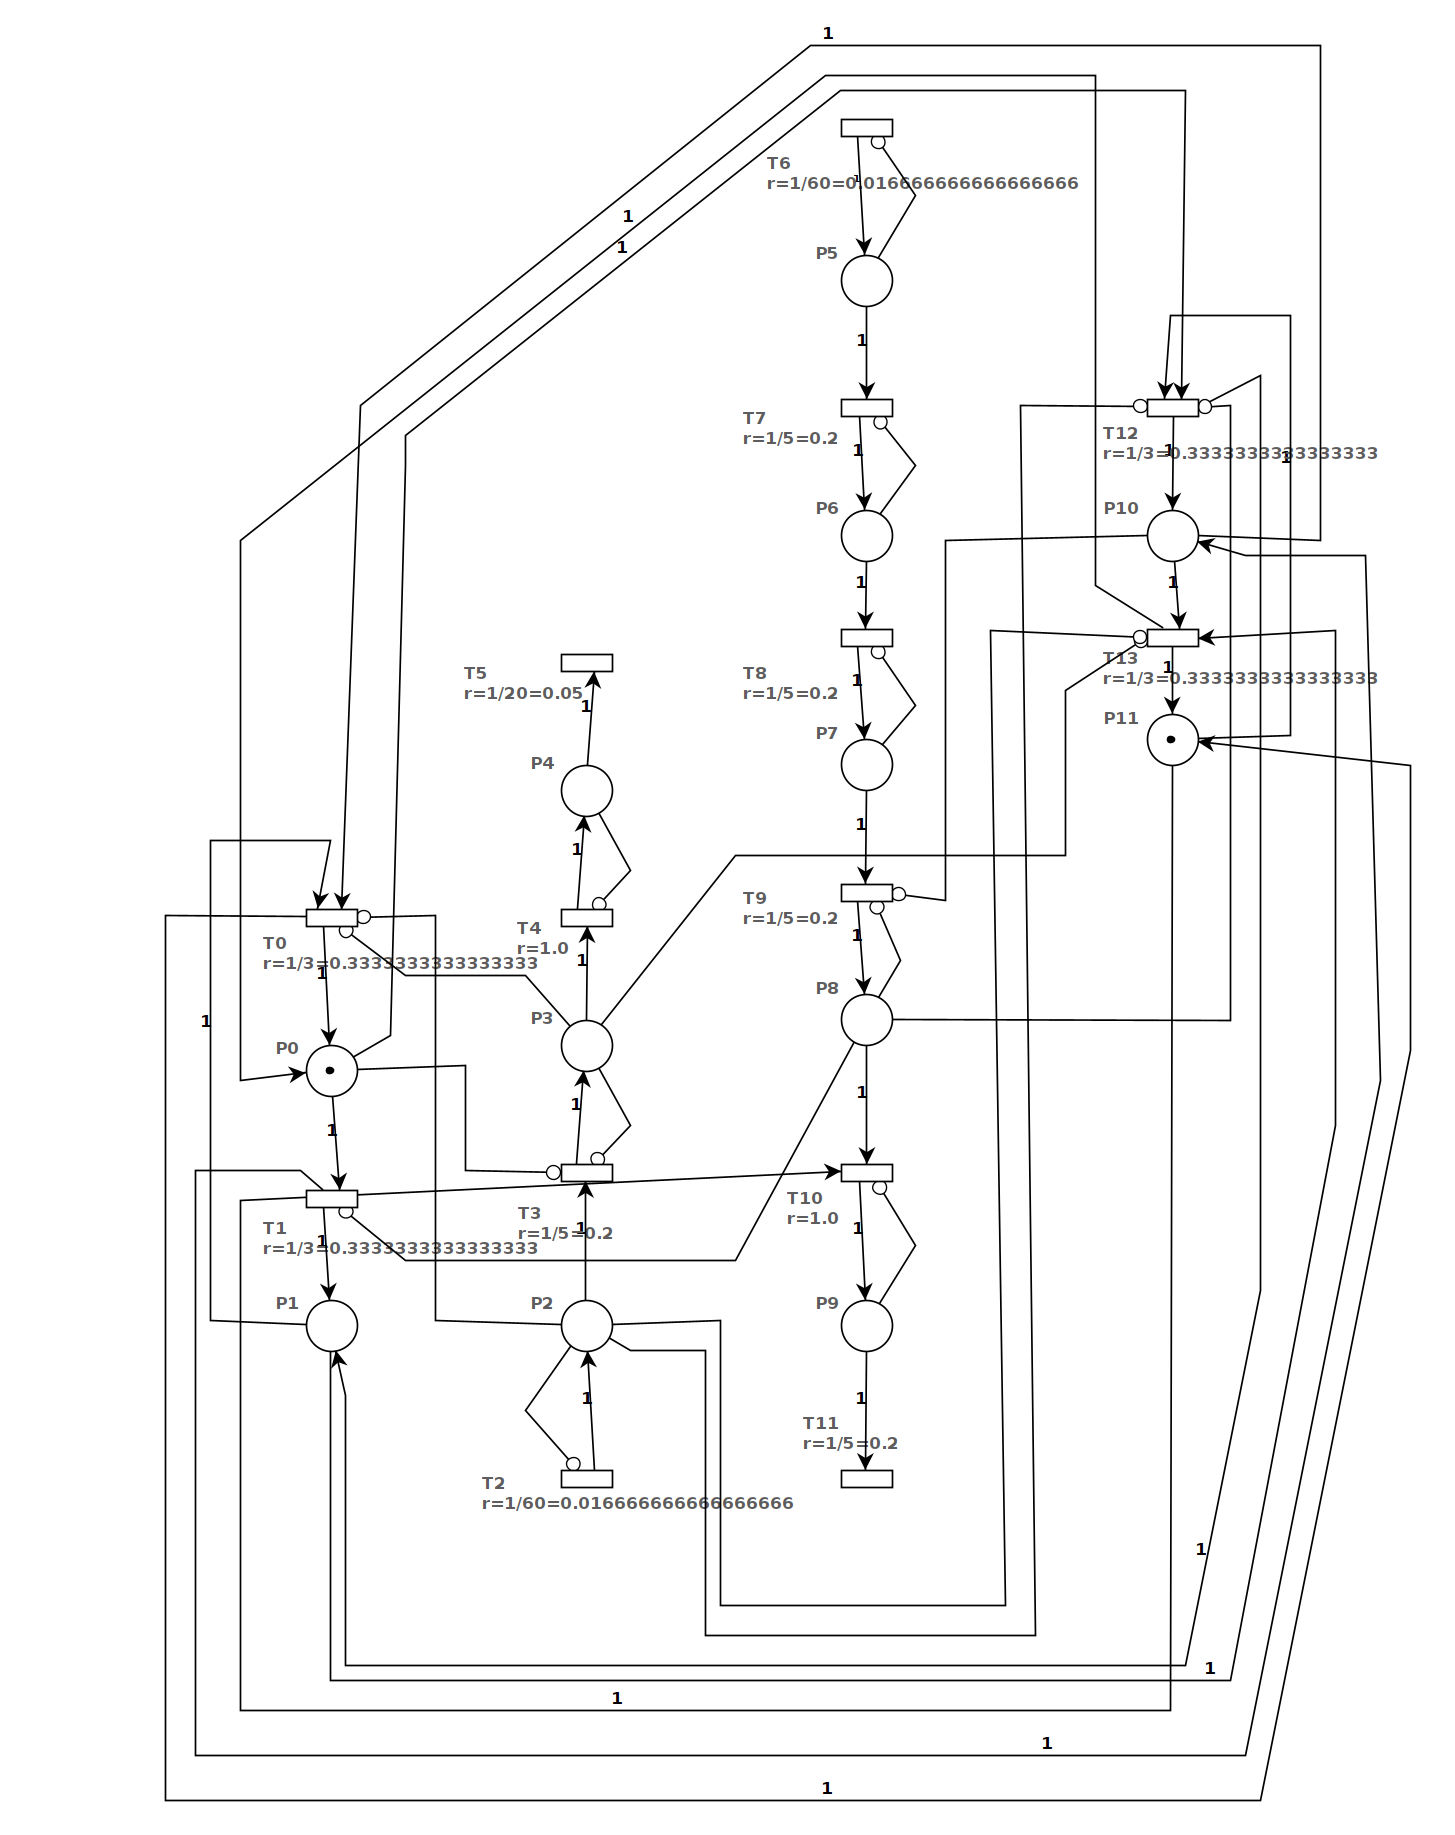
\includegraphics[width=0.85\linewidth]{../../lab10/ex_1}
    \caption{Semafory naprzemienne. Nie można przełączyć automatycznie z $p_{11}$ na $p_{10}$ semafora prawego, kiedy w $p_{2}$ pojawi się tramwaj.}
\end{figure}

\clearpage

\ex{Przebudowa sieci}
\begin{figure}[H]
    \centering
    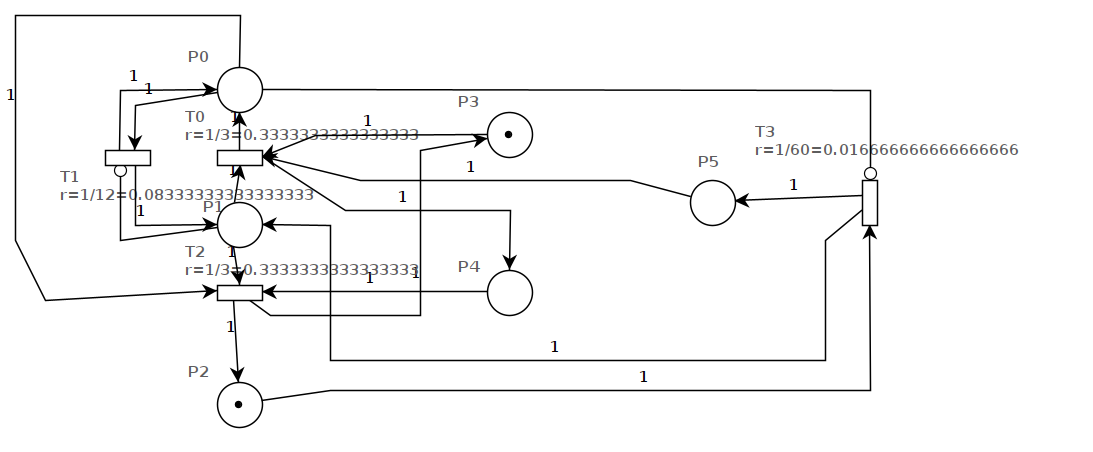
\includegraphics[width=\linewidth]{../../lab10/ex_2}
    \caption{Sieć symulująca sygnalizację świetlną.}
\end{figure}

Pierwotnie w tej sieci do odpalenia na raz było możliwe tylko jedno przejście, więc
wartości prawdopodbieństwa wynikają bezpośrednio z $\lambda$ przejść($r$).

\begin{table}[H]
    \centering
    \begin{tabularx}{\linewidth}{Xl}
        \hline
        Intensywności odpalania                          &
        $\Lambda = \{\frac{1}{3},\frac{1}{12},\frac{1}{3},\frac{1}{60}\}$                 \\
        \hline
        Prawdopodobieństwo odpalenia czasowego przejścia &
        $\{Pr_i: i\in[0,1,2,3]\} = \{\frac{1}{3},\frac{1}{12},\frac{1}{3},\frac{1}{60}\}$ \\
        \hline
        Średni czas odpalenia czasowego przejścia        &
        $\{T(t_i): i\in[0,1,2,3]\} = \{3,12,3,60\}$                                       \\
        \hline
        Średni czas przebywania w oznakowaniu            &
        $\{T(M_j): i\in[0,1,2,3]\} = \{3,12,3,60\}$                                       \\
        \hline
    \end{tabularx}
\end{table}

\end{document}